%Here, we provide background on energy harvesting systems and the intermittent software execution model. We then discuss the key limitations of existing task-based execution models for intermittent computing that \sys addresses.

%\begin{figure}
\begin{wrapfigure}{t!}{0.5\textwidth}
	\begin{subfigure}[t]{\linewidth}
		\centering 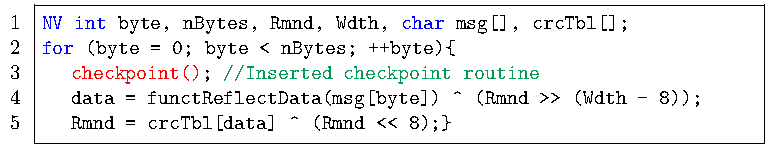
\includegraphics[width=\columnwidth]{figures/crc_example}
		\caption{Simplified C code snippet of a CRC calculation from~\cite{hicks_mibench2_2016}: per-byte message division by a polynomial; \texttt{NV} denotes non-volatile variable declaration.}\label{fig:crc_example}
	\end{subfigure}
	\begin{subfigure}[t]{\linewidth}
		\centering 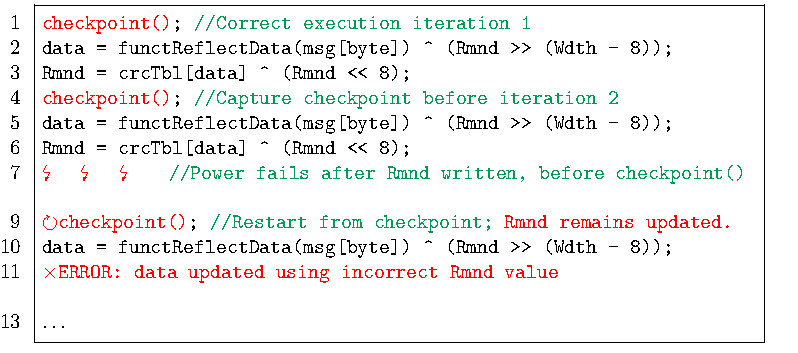
\includegraphics[width=\columnwidth]{figures/crc_example_war}
		\caption{Execution steps of the loop body in the snippet above: non-volatile checkpointing did not guarantee data consistency as data has been manipulated (line 9) with stale reminder (line 3)}\label{fig:crc_example_war}
	\end{subfigure}
	\caption{Code example demonstrating checkpointing gives rise to data inconsistency.}\label{fig:code_demo_incosistency}
\end{wrapfigure}
%\end{figure}

\subsection{Energy Harvesting Systems}
\label{sec:background_harvesting}

Energy harvesting devices operate using energy extracted from sources such as radio frequency transmissions and solar energy. These devices elide tethered power or a battery, instead collecting energy into a capacitor, operating when sufficient energy accumulates, and upon depleting the energy, turning off and recharging.
%\TODO{We need a figure that shows what intermittent execution looks like.}
%
%Batteryless operation has a number of important advantages, making intermittent computing an important research domain. Supplying power to billions~\cite{gartner_iot} of embedded computers using batteries is not sustainable. The European Commission estimates that more than 160 kilotons of consumer batteries enter the European Union annually~\cite{eu_batteries_2016}. Batteries are an environmental risk, are fragile, are limited in their number of charge/discharge cycles, and may require costly physical maintenance that is difficult or impossible deployed (e.g. in space~\cite{kicksat}). By contrast, super-capacitors are durable, promising millions of charge/discharge cycles~\cite[Sec. I]{ongaro_pwre_2012}. The main limitation in moving to capacitor-based energy storage is that capacitor energy density---and consequently operating discharge time---is orders of magnitude less than a battery. 
%
%Given current technology development, battery-less systems are best suited for very long-term sensing and monitoring where access to recharge is either prohibitive or impossible. These include battery-less image capture and processing~\cite{naderiparizi_rfid_2015}, animal monitoring~\cite{thomas_jbcs_2012} or implantable~\cite{rodriguez_tbcs_2015} and digestible~\cite{nadeau_naturebio_2017} sensors.
%
There are several energy harvesting battery-less hardware platforms. For instance, computational RFIDs---open-source TI MSP430-based~\cite{wolverine} WISP~\cite{wisp5} (with its variants such as WISPCam~\cite{naderiparizi_rfid_2015}, NFC-WISP~\cite{zhao_rfid_2015} or NeuralWISP~\cite{holleman_biocas_2008}), Moo~\cite{moo}, and commercial ones such as~\cite{medusa_farsens_2017}. Other platforms include ambient backscatter tag~\cite{liu_sigcomm_2013,parks_sigcomm_2014} or battery-less phone~\cite{talla_imwut_2017}. 

%In all of the above, the main source of energy harvested is the electromagnetic radiation in the radio frequency range (ambient transmitters such as high power TV transmitters~\cite{liu_sigcomm_2013} or dedicated RFID antenna~\cite{wisp5,moo,talla_imwut_2017,medusa_farsens_2017,holleman_biocas_2008,naderiparizi_rfid_2015}). Naturally, other forms of energy harvesting sources exist, including temperature gradient, (micro-)motions, light/sun radiation, vibrations, and body fluid flow (blood, gastric acid). Several recent surveys discussing energy harvesting, low-power, embedded systems and intermittent computing at a high level~\cite{paradiso_pvc_2005,soyata_csm_2016,prasad_comst_2014,ku_cst_2016,lucia_snapl_2017}.

\textbf{Hardware Assumptions.} \sys is designed for the demands of existing and future energy-harvesting platforms based around general purpose, commodity computing components~\cite{wisp,msp430datasheet}. We assume a device with a memory system that has fast, byte-addressable volatile and non-volatile memory; in particular, our target platform, WISP~\cite{wisp}, is equipped with a mixture of SRAM and FRAM. Our implementation leverages hardware support for fast, bulk-copying between memories via DMA~\cite{msp430datasheet}. We do not require a particular non-volatile memory technology, nor do we require architectural additions commodity processors~\cite{su_date_2017,ratchet,quickrecall,nvp}. \sys supports I/O behavior similar to~\cite{alpaca,chain}, allowing safe, synchronous I/O and unsafe, asynchronous I/O.

\subsection{Intermittent Execution}
\label{sec:background_consistency}

%\textcolor{red}{reference work by Intel~\cite{baghsorkhi_cgo_2018}}

%Energy-harvesting devices execute software according to the {\em intermittent execution model}. Physically, a device charges until a threshold, operates briefly until its energy is depleted, shuts down recharges, and repeats the cycle.
%
Software running on an energy-harvesting device executes {\em intermittently} because energy sources are not always available to harvest and buffer sufficient operational energy. An intermittent execution is composed of operating periods interspersed with power failures~\cite{dino,chain,alpaca,ratchet}. The frequency of failures depends on the size of the device's energy storage buffer: a larger buffer allows longer operating periods. 
%Energy-harvesters provide input power orders of magnitude less than operating power, making recharging negligible during operation.
%Intermittent execution is different from continuous execution. 
A power failure clears volatile  state (registers, stack, and globals) and non-volatile memory (e.g., FRAM) persists. Upon a power failure, control flows to a prior point in the execution: by default, to the beginning of {\tt main()}. Early intermittent systems preserved progress by periodically checkpointing volatile execution context to non-volatile memory~\cite{mementos}, sometimes using hardware support~\cite{mementos,mottola2017harvos,hibernusplusplus,hibernus,idetic,quickrecall}. 

%\begin{figure}
%	\centering
%	\subfloat[Simplified C code snippet of a CRC calculation from~\cite{hicks_mibench2_2016}: per-byte message division by a polynomial; \texttt{NV} denotes non-volatile variable declaration]{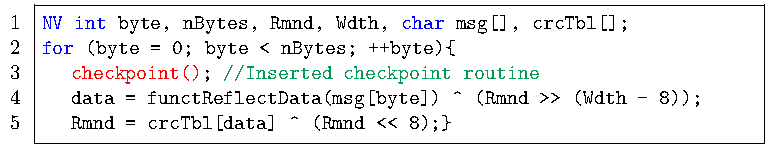
\includegraphics[width=\columnwidth]{figures/crc_example}\label{fig:crc_example}}\\
%	\subfloat[Consecutive execution steps of the loop body in the snippet above: non-volatile checkpointing did not guarantee data consistency as data has been manipulated (line 9) with stale reminder (line 3)]{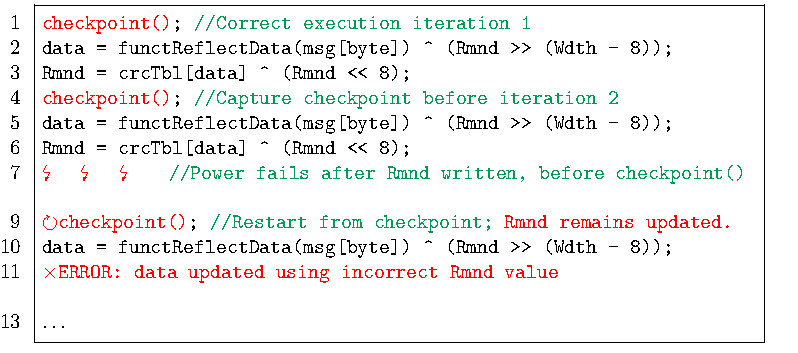
\includegraphics[width=\columnwidth]{figures/crc_example_war}\label{fig:crc_example_war}}
%	\caption{Code example demonstrating effect of write after read on volatile memory checkpointing.}
%	\label{fig:code_demo_incosistency}
%\end{figure}

Checkpoints of volatile state preserve intermittent progress, but do not ensure data consistency~\cite{dino,chain,ratchet}. Data may become inconsistent if an attempt to execute some computation {\em writes} to a non-volatile variable, then power fails, then a second attempt to re-execute the same computation incorrectly {\em reads} the value written in the first attempt, rather than the variable's original value. The situation occurs when code includes a \emph{write-after-read} (WAR) dependence between operations that manipulate non-volatile variables~\cite{ratchet,dino,alpaca}---see Figure~\ref{fig:code_demo_incosistency} that illustrates how state can become inconsistent in an intermittent execution using the cyclic redundancy check (CRC) code from MIBench2~\cite{hicks_mibench2_2016}.
%Figure~\ref{fig:code_demo_incosistency} illgit statuustrates how state can become inconsistent in an intermittent execution using the cyclic redundancy check (CRC) code from MIBench2~\cite{hicks_mibench2_2016}. The code computes the CRC for an $\texttt{nBytes}$ byte message $\texttt{msg}$ with remainder $\texttt{Rmnd}$.
%Despite checkpointing at line 3 in Fig.~\ref{fig:crc_example}, the code may compute  $\texttt{data}$ incorrectly because of the read of $\texttt{Rmnd}$ on line 4 and the write of $\texttt{Rmnd}$ on line 5. Figure~\ref{fig:crc_example_war} shows an intermittent execution. The second iteration writes $\texttt{Rmnd}$, but power fails before the checkpoint. After restarting, line 9 reads the updated value of $\texttt{Rmnd}$, producing an incorrect $\texttt{data}$ value. Checkpoint-based systems risk violating memory consistency~\cite{dino}. 
To maintain consistency, prior systems~\cite{dino,ratchet} {\em version} a subset of non-volatile data with the checkpoint. Task-based systems~\cite{chain,alpaca}, which we focus on, ensure consistency using programmer, compiler, and runtime support.

\subsection{Task-based Intermittent Programming}
\label{section:background_task_computing}

Task-based execution models~\cite{dino,chain,alpaca} ask the programmer to decompose their program into tasks. A task is a function with no caller containing arbitrary computation, sensing, and communication. A programmer describes task control-flow as a {\em task graph}. Task flow happens at programmer demarcated transition points that may be conditional on program values. 
%Task-based programming abstractions guarantee that tasks execute {\em atomically}, regardless of power failures. 
Task-based runtime systems ensure task-atomic semantics by ensuring that repeated task executions are idempotent. The key to idempotence is ensuring that non-volatile updates made by an interrupted task are never visible to a future task execution.  

There are several run time strategies to ensuring task idempotence. One approach~\cite{alpaca}, is to identify non-volatile data involved in WAR dependences in a task (like DINO~\cite{dino} and Ratchet~\cite{ratchet} did for checkpoints), execute the task using private copies of those data, and commit the private copies on task completion. Another way is to statically create multiple versions of non-volatile data shared by tasks and ensure that no task reads and writes the same version~\cite{chain}. Regardless of the strategy, task-based systems execute statically-defined tasks atomically, completing in one or more attempt. 

\subsubsection{Costs of Task-based Models}
\label{sec:cost_task-based}

Despite their advantages, the task-based programming models have their limitations. Two major ones being: {\em memory consistency enforcement overhead} and {\em inflexibility to dynamic energy harvesting conditions}.

\begin{table}
	\centering
	\footnotesize
	\begin{tabular}{|c|c|}
		\hline
		Model & Data Copied to/from NVRAM \\
		\hline\hline
		Mementos~\cite{mementos}	& Registers + Stack     \\
		DINO~\cite{dino}	& Registers + WAR variables \\
		Chain~\cite{chain}	& PC + channel data\\
		Alpaca~\cite{alpaca}	& PC + WAR variables \\
		Ratchet~\cite{ratchet}, Clank~\cite{hicks_isca_2017} & Registers (requires NV main memory) \\
		Region Formation~\cite{baghsorkhi_cgo_2018} & \textcolor{red}{XXX} \\
		\hline
	\end{tabular}
	\caption{Memory consistency enforcement overheads of intermittent execution models; \emph{PC}: program counter, \emph{channel data}: variables explicitly task-shared by the programmer, \emph{WAR variables}: variables involved in WAR dependences (\emph{NV}: non-volatile). \todo{region formation}{Alexei}}
	\label{table:chechpoint_comparison}
\end{table}


\textbf{Memory Consistency Enforcement Overhead.} Intermittent execution models incur overheads to checkpoint data~\cite{dino,ratchet,quickrecall,mementos}, manage channels~\cite{chain}, or privatize and commit data~\cite{alpaca}. Table~\ref{table:chechpoint_comparison} compares overheads for recent intermittent execution models (cf. \cite[Sec. 2.4]{alpaca}.) The mechanism responsible for overhead in each model varies, but the bulk of overhead in all models is a manipulating non-volatile memory. Checkpointing moves data to and from non-volatile memory, channel accesses manipulate non-volatile data~\cite{chain}, privatization copies from and commits to non-volatile memory~\cite{alpaca}, and idempotence solutions~\cite{ratchet} use {\em only} non-volatile memory.  
% We do not need to emphasize the following figure! (Sinan)
%\begin{figure}
%\begin{subfigure}[t]{.49\columnwidth}
%	\centering 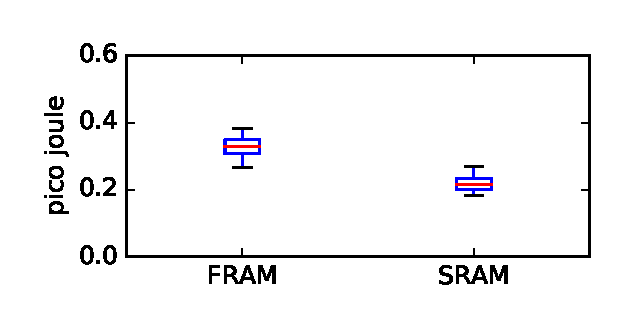
\includegraphics[width=\columnwidth]{figures/fram_write}
%	\caption{Cost of \emph{write} operation}
%\end{subfigure}%
%\begin{subfigure}[t]{.49\columnwidth}
%	\centering 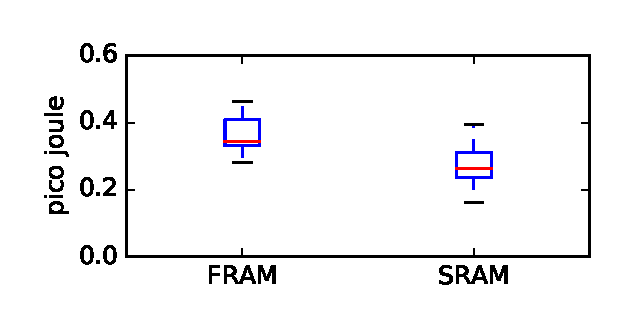
\includegraphics[width=\columnwidth]{figures/fram_read}
%	\caption{Cost of \emph{read} operation}
%\end{subfigure}
%	\caption{\textbf{Cost of accessing volatile (SRAM)/non-volatile (FRAM) memory during write/read operation.} \textcolor{red}{figures need to be merged into one}}\label{fig:framEnergy}
%\end{figure}
To understand the non-volatile memory access overheads, we measured the energy consumption of volatile (SRAM) and non-volatile (FRAM) memory operations for the MSP430FR5969~\cite{msp430datasheet} MCU. We used EDB~\cite{edb} to monitor voltage drop on a capacitor powering the device across 1600 read and write accesses to each memory type, randomizing to avoid caching. Our experiment showed that a non-volatile memory access consumes around 1.5 times the energy of a volatile access.
%~\cite{}. \todo{add citation to TI specification on FRAM energy cost}{Przemek}. 
% Figure~\ref{fig:framEnergy} summarizes the data, showing that a non-volatile memory access consumes around 1.5 times the energy of a volatile access in this device. This observation is also consistent with the TI specification~\cite{}. \todo{add citation to TI specification on FRAM energy cost}{Przemek} 
Based on this observation, one of the primary motivation of \sys is to promote accessing SRAM more frequently rather than FRAM in order to reduce memory access energy overhead and to increase the time between power failures. 

%The cost of non-volatile memory motivates \sys, which virtualizes memory to primarily use SRAM.

%The above result reassures the intuitive observation that a decrease of checkpoint frequency (CP) decreases the energy cost associated with each state preservation method and reduces operation cost which in most simplistic terms is defined as $\mathcal{O}(\text{CP})+\mathcal{O}(\text{PL})$, where PL is the cost of program execution without checkpointing. On the other hand, this increases task/checkpoint re-execution time. The ideal solution is a runtime that \emph{adaptively} changes task size during runtime, which however exposes a second problem.

%\begin{table}
%	\centering
%	\footnotesize
%	\begin{tabular}{|c|c|}
%		\hline
%		Platform name & Storage capacitor size \\
%		\hline \hline
%		%Moo~\cite{moo} & 0.1\,F \\
%		WISPCam~\cite{naderiparizi_rfid_2015} & 6.08\,mF \\ %tested [11.24, 17.45, 21.98]\,mF
%		%NFC-WISP~\cite{zhao_rfid_2015} & 300\,$\mu$F \\
%		NeuralWISP~\cite{holleman_biocas_2008} & 100\,$\mu$F \\
%		WISP~\cite{wisp5} & 47\,$\mu$F \\
%		{\em BioImpedance} sensor~\cite{rodriguez_tbcs_2015} & 20\,$\mu$F \\
%		{\em Ingestible} sensor~\cite{nadeau_naturebio_2017} & 220\,$\mu$F\\
%		\hline
%	\end{tabular} 
%	\caption{{\em Default} energy storage sizes for example battery-less platforms. Observe a huge variation in storage capacity.}
%	%We note that values for other representative platforms~\cite{medusa_farsens_2017,talla_imwut_2017,liu_sigcomm_2013,parks_sigcomm_2014} were not reported in their respective papers.
%	\label{table:capacitor}
%\end{table}

%Przemek placeholder
%\textbf{Task-based Models have Syntactic Limitations.} State of the art task-based programming models, Alpaca~\cite{alpaca}, has substantial limitations that prohibit writing generic programs. First, for Alpaca (and Chain~\cite{chain}), accesses to protected variables must be applied \emph{only} by using the variable's name, i.e. reference by variable address is not possible. This limitation implies that existing third-party libraries, such as MCU-tailored FFT library~\cite{}, cannot be implemented to support Alpaca or Chain (not to mention the impossibility of the development of an intermittent-safe \texttt{memcpy}). Furthermore, if a protected variable needs to be accessed in a code path that is not predictable by the compiler, for instance an Interrupt Service Routine, Alpaca cannot protect that access.

\textbf{Fixed-size Tasks are Inflexible and Inefficient.} If a programmer writes a task that consumes {\em more} energy than the device can buffer, the task will never complete using buffered energy {\em preventing forward progress} by repeatedly re-executing. If a programmer writes tasks that consume far {\em less} energy than a device can buffer, the system may operate {\em inefficiently}. When a task and its successor both complete, the two tasks were interleaved by a task boundary that preserves progress and state (i.e., checkpoint or commit). However, absent a power failure, the work to preserve state was {\em unnecessary}, incurring overhead on the tasks' executions. Avoiding excessively costly, non-terminating tasks and short, high-overhead tasks is a programming challenge, given fixed hardware (no support from dedicated circuitry to measure the state of energy buffer) with a fixed energy buffering capacity. Buffer sizes from prior work on intermittently-powered computing hardware vary widely from 20\,$\mu $F~\cite{rodriguez_tbcs_2015} to 0.1\,F~\cite{moo}. Sizing tasks complicates {\em porting} code from one device to another. An excessively costly task on a device with a small energy buffer may be a relatively short task on a device with a larger buffer. The key problem is that using existing systems, by defining tasks statically for a fixed energy buffer, the programmer either risks non-termination or poor performance due to high overhead. \sys's execution model based on {\em task coalescing} and {\em task downscaling}.  Coalescing dynamically merges multiple tasks based on execution behavior to amortize the cost of committing each task separately. Downscaling breaks up a single task into multiple subtasks that commit individually to avoid executing a single task that is too large to complete using the device's buffered energy.  Section~\ref{sec:task_adaptation}describes \sys's adaptive coalescing and downscaling mechanisms in detail. The main enabler for \sys's adaptation is its novel \emph{memory virtualization} mechanism, which is described in Section~\ref{sec:memory_virtulaization}.

%\textbf{Motivating the Design of \sys's Execution Model.} The challenge of \em{efficiently} executing a program under frequent power failures, lies in the fact the the program needs to be energy aware. This challenge becomes even bigger when \em{generality} is a design requirement and such the system must not require a specific hardware circuitry to offer its efficiency. \em{Fllexibility} is key for wide adaptation, therefore, \sys's execution model should not limit the programmer to a subset of the functionality of the underlying software technology. \em{\sys champions an efficient, general, and flexible intermittent execution.}
